\chapter{The Euler-Bernoulli Beam Theory with Governing Equations}
\label{sec:second}

A beam is a structural element having one dimension that is much larger than the other two and capable 
of resisting the loads applied laterally to the beam axis. Since the further investigations are pursued
for the Euler-Bernoulli beam theory, known as thin beam theory, the main assumptions and the governing 
equations of the Euler-Bernoulli are given in more detail.

\section{Assumptions of the Euler-Bernoulli Beams}

The main hypothesis of the Euler-Bernoulli beam theory is that plane cross-sections which are orthogonal 
to the beam axis (neutral axis) stay still plane and orthogonal to the beam axis after deformation. 
The overall assumptions of the Euler beam theory: %\ref{fig:euler_theory}

\begin{itemize}
    \item Plane cross-sections remain plane and perpendicular to the neutral axis of the beam after deformation.
    \item The deformations are small, so the equilibrium is computed on the reference configuration (Small deformation theory).
    \item Behavior of the beam is linear elastic and isotropic.
    \item Shear strains are neglected.
\end{itemize}


\begin{figure}[!ht]
    \centering
    \includegraphics[scale=0.5]{beam_theory.png}  
    \caption{The Euler-Bernoulli and Timoshenko beam deflections}
    \label{fig:euler_theory}
\end{figure}

As depicted in Fig. \ref{fig:euler_theory}, the plane cross-sections stay plane and perpendicular to the 
beam axis in the Euler-Bernoulli beam. In the Timoshenko beam, plane cross-sections still remain plane but
are no longer perpendicular to the beam axis. The difference between normal to the beam axis and plane
cross-section is known as shear deformation. Here, shear strains will be ignored so the beam Formulation
is considered under the Euler-Bernoulli beam theory, which is known also as thin beam theory.

\section{Governing Equations}

\subsection{Time-dependent beam equation}

Consider the governing equation of an Euler-Bernoulli beam under 
the space-time dependent distributed load as (Fig. \ref{fig:beam_arbitrary})

\begin{equation}
    \label{eq:pde_time}
    \rho A \frac{\partial^{2} w(x,t)}{\partial t^{2}} + \frac{\partial^{2}}{\partial x^{2}}\left(E I \frac{\partial^{2} w(x,t)}{\partial x^{2}}\right) + q(x, t) = 0, x \in \Omega, t \in [0,T]
\end{equation}


\noindent where $w(x,t)$ is the unknown solution, $\Omega$ is a subset of $\mathbb{R}^{D}$,
$E$ is the uniform elastic modulus of the material, 
$I$ is the moment of the inertia of the cross-section of the beam, $\rho$
is the material density, $A$ is the cross-sectional area, and $q(x,t)$ is distributed space-time varying load. 
Eq. \ref{eq:pde_time} is known as also 
\textit{Euler-Langrange} equation \cite{wang2007vibration} used mainly in vibration problems. The first term
describes the dissipated kinetic energy where $\rho A$ is area density or the mass per unit length, 
and the second term characterizes the potential energy due to internal forces. 

\vspace{3mm}

\noindent The concentrated load $q$ can be considered as a special case of the distributed load as follows:

\begin{equation}
    \label{eq:load_time}
    q(x,t) = P(t)\delta\left(x-x_{0}\right)
\end{equation}

\noindent where $\delta$ is the \textit{Dirac} delta function, and $P(t)$ is the time-dependent load applied
at position $x_{0}$.



\begin{figure}[!ht]
    \centering
    \includegraphics[scale=0.7]{beam_arbitrary.png}  
    \caption{A fixed-fixed supported beam under a space-time dependent distributed load.}
    \label{fig:beam_arbitrary}
\end{figure}

\subsection{Static beam equation}

Eliminating time terms in Eqs. \ref{eq:pde_time} and \ref{eq:load_time}, the governing ordinary differential equation
is obtained for a static model

\begin{equation}
    \label{eq:ode_space}
    \frac{\partial^{2}}{\partial x^{2}}\left(E I \frac{\partial^{2} w(x)}{\partial x^{2}}\right) + q(x) = 0, x \in \Omega,
\end{equation}

\noindent and, similarly if $q(x)$ is a concentrated load

\begin{equation}
    q(x) = P \delta\left(x-x_{0}\right).
\end{equation}


\section{Boundary Conditions and Beam Supports}

To estimate the unknown solution $w(x,t)$, 
the governing equation of the Euler-Bernoulli beam 
must be solved using the initial and boundary conditions. Since the governing equation is of the $4th$ order in space (Eq. \ref{eq:pde_time}), 
four different boundary conditions are introduced:
\begin{itemize}
    \item $w(x,t) \rightarrow$ represents the displacement in the z direction,
    \item $w_{x}(x,t) \rightarrow$ indicates the slope of the beam,
    \item $w_{xx}(x,t) \rightarrow$ measures the bending moment,
    \item $w_{xxx}(x,t) \rightarrow$ measures the shear force, 
\end{itemize}

\noindent at location $x \in \Omega$ and time $t \in [0,T]$. 

Similary, and two initial conditions are needed as Eq. \ref{eq:pde_time} is of the $2^{th}$ order in time
\begin{itemize}
    \item $w(x,0) \rightarrow$ represents the displacement in the z direction,
    \item $w_{t}(x,0) \rightarrow$  indicates the time derivative of the displacement,
\end{itemize}

\noindent at location $x \in \Omega$ and at time $t=0$. Initial conditions are not taken 
into account in the static beam equation since the time-dependent derivative term vanishes. 

\vspace{5mm}
\noindent Two main supports will be further investigated:
\begin{itemize}
    \item fixed supported beams
    \item simply supported beams
\end{itemize}

\subsection{Cantilever beam}

A cantilever beam is fixed supported at one end and free at the other as depicted in Fig. \ref{fig:beam_cantilever}. 
No displacement and rotation are allowed at the fixed edge. No bending moment and no shear force at the free edge
are generated. 

\begin{figure}[!ht]
    \centering
    \includegraphics[scale=0.6]{beam_cantilever.png}  
    \caption{An illustration of a fixed supported beam}
    \label{fig:beam_cantilever}
\end{figure}

Boundary conditions of a cantilever beam
\begin{equation}
    \begin{array}{l}
    w(x,t)=0 \quad and \quad w_{x}(x,t)=0, \quad at \; x=0, t=[0,T] \\
    w_{xx}(x,t)=0 \quad and \quad w_{xxx}(x,t)=0, \quad at \; x=L, t=[0,T]
    \end{array}
\end{equation}

\subsection{Simply supported beam}
Simply supported beam is pinned at the ends for two edges as shown in Fig. \ref{fig:beam_pinn}. At both pinned ends, 
no displacement but rotation 
is allowed which means that no bending moments are generated.

\vspace{5mm}

\begin{figure}[!ht]
    \centering
    \includegraphics[scale=0.6]{beam_pinn.png}  
    \caption{An illustration of a simply supported beam.}
    \label{fig:beam_pinn}
\end{figure}

Boundary conditions of a simply supported beam
\begin{equation}
    \label{eq:simply_supported_bc}
    \begin{array}{l}
    w(x,t)=0 \quad and \quad w_{xx}(x,t)=0, \quad at \; x=0, t=[0,T] \\
    w(x,t)=0 \quad and \quad w_{xx}(x,t)=0, \quad at \; x=L, t=[0,T]
    \end{array}
\end{equation}

\subsection{Clamped beam}
A clamped beam is fixed supported at both ends as depicted in Fig. \ref{fig:beam_clamped}. At both fixed ends,
no displacement and rotation is allowed. 

\begin{figure}[!ht]
    \centering
    \includegraphics[scale=0.6]{beam_clamped.png}  
    \caption{An illustration of a clamped beam.}
    \label{fig:beam_clamped}
\end{figure}

Boundary conditions of a clamped beam
\begin{equation}
    \begin{array}{l}
    w(x,t)=0 \quad and \quad w_{x}(x,t)=0, \quad at \; x=0, t=[0,T] \\
    w(x,t)=0 \quad and \quad w_{x}(x,t)=0, \quad at \; x=L, t=[0,T]
    \end{array}
\end{equation}
